\documentclass[10pt,a5paper]{extarticle}
\usepackage[margin=.8cm]{geometry}
\usepackage[utf8]{inputenc}
\usepackage[IL2]{fontenc}
\usepackage[czech]{babel}
\usepackage{microtype}
\usepackage{amssymb}
\usepackage{amsthm}
\usepackage{amsmath}
\usepackage{xcolor}
\usepackage{graphicx}
\usepackage{wasysym}
\usepackage{multicol}

\usepackage[inline]{enumitem}

\newcommand{\R}{\mathbb{R}}

\newcommand{\hint}[1]{{\color{gray}\footnotesize\noindent(Nápověda: #1)}}

\setlist[enumerate]{label={(\alph*)},topsep=\smallskipamount,itemsep=\smallskipamount,parsep=0pt,itemjoin={\quad}}
\setlist[itemize]{topsep=\smallskipamount,noitemsep}

\def\tisk{%
\newbox\shipouthackbox
\pdfpagewidth=2\pdfpagewidth
\let\oldshipout=\shipout
\def\shipout{\afterassignment\zdvojtmp \setbox\shipouthackbox=}%
\def\zdvojtmp{\aftergroup\zdvoj}%
\def\zdvoj{%
    \oldshipout\vbox{\hbox{%
        \copy\shipouthackbox
        \hskip\dimexpr .5\pdfpagewidth-\wd\shipouthackbox\relax
        \box\shipouthackbox
    }}%
}}%

\let\results\newpage
\let\endresults\relax

\def\resultssame{%
    \long\def\results##1\endresults{%
        %\vfill
        \noindent\rotatebox{180}{\vbox{##1}}%
    }%
}


\newtheorem*{poz}{Pozorování}

\theoremstyle{definition}
\newtheorem{uloha}{\atr Úloha}
\newtheorem{suloha}[uloha]{\llap{$\star$ }Úloha}
\newtheorem*{bonus}{Bonus}
\newtheorem*{defn}{Definice}

\pagestyle{empty}

\let\ee\expandafter

\def\vysld{}
\let\printvysl\relax

\makeatletter
\long\def\vyslplain#1{\ee\ee\ee\gdef\ee\ee\ee\vysld\ee\ee\ee{\ee\vysld\ee\printvysl\ee{\the\c@uloha}{#1}}}
\let\vysl\vyslplain

\def\locvysl#1{\ee\gdef\ee\locvysld\ee{\locvysld\item #1}}
\let\lv\locvysl

\newenvironment{ulohav}[1][]{\begin{uloha}[#1]\gdef\locvysld{\begin{enumerate*}}}{\ee\vyslplain\ee{\locvysld\end{enumerate*}}\end{uloha}}
\def\stitem{\@noitemargtrue\@item[$\star$ \@itemlabel]}

\makeatother

\def\atr{}
\def\basic{\def\atr{\llap{\mdseries$\sun$ }\gdef\atr{}}}
\def\interest{\def\atr{\llap{$\star$ }\gdef\atr{}}}
\def\iinterest{\def\atr{\llap{$\star\star$ }\gdef\atr{}}}
\let\mb\mathbf



\begin{document}

%\tisk
%\resultssame

\section*{27. Úvod do posloupností}

\begin{ulohav}
U následujících rekurentních předpisů odhadněte, jaký bude předpis pro $n$-tý člen, a svůj odhad ověřte:
\vskip-1.5\bigskipamount\vbox{}
\begin{multicols}{2}
\begin{enumerate}
    \item $a_1 = 4$, $a_n = a_{n-1} + 3$ pro $n > 1$\lv{$3n+1$}
    \item $a_1 = 1$, $a_n = -a_{n-1}$ pro $n > 1$\lv{$(-1)^{n+1}$}
    \item $a_1 = 2$, $a_n = \sqrt{a_{n-1}}$ pro $n > 1$\lv{$2^{2^{1-n}}$}
    \item $a_1 = 3$, $a_n = 2 a_{n-1}$ pro $n > 1$\lv{$3\cdot 2^{n-1}$}
    \item $a_1 = 3$, $a_n = 2 a_{n-1} - 1$ pro $n > 1$\lv{$2^n + 1$}
    \item $a_1 = 1$, $a_n = 2 a_{n-1} - 1$ pro $n > 1$\lv{$1$}
    \item $a_1 = -3$, $a_n = 2 a_{n-1} + n$ pro $n > 1$\lv{$-n-2$}
    \stitem $a_1 = 3$, $a_n = -2 a_{n-1} + 3$ pro $n > 1$\lv{$1-(-2)^n$}
    \item $a_1 = 1$, $a_2 = 4$, $a_n = 2a_{n-1} - a_{n-2}$ pro $n>2$\lv{$3n-2$}
    \stitem $a_1 = 2$, $a_2 = 8$, $a_n = 4a_{n-1} - 4a_{n-2}$ pro $n>2$\lv{$n \cdot 2^n$}
\end{enumerate}
\end{multicols}
\end{ulohav}


\begin{ulohav}
Dopočtěte první dva členy posloupnosti, jestliže o ní víme
\begin{enumerate}
    \item $a_{n} = 2a_{n-1} - n$ pro $n>1$, $a_3=33$\lv{$a_1 = 10$, $a_2 = 18$}
    \item $a_{n} = a_{n-1} + a_{n-2}$ pro $n>2$, $a_5=3$, $a_6=4$\lv{$a_1 = 3$, $a_2 = -1$}
\end{enumerate}
\end{ulohav}


\begin{ulohav}
Napište rekurentní předpisy pro následující posloupnosti \uv{zadané obrázkem}:\par
\begin{flushleft}
\begin{enumerate*}
    \item $\vcenter{\hbox{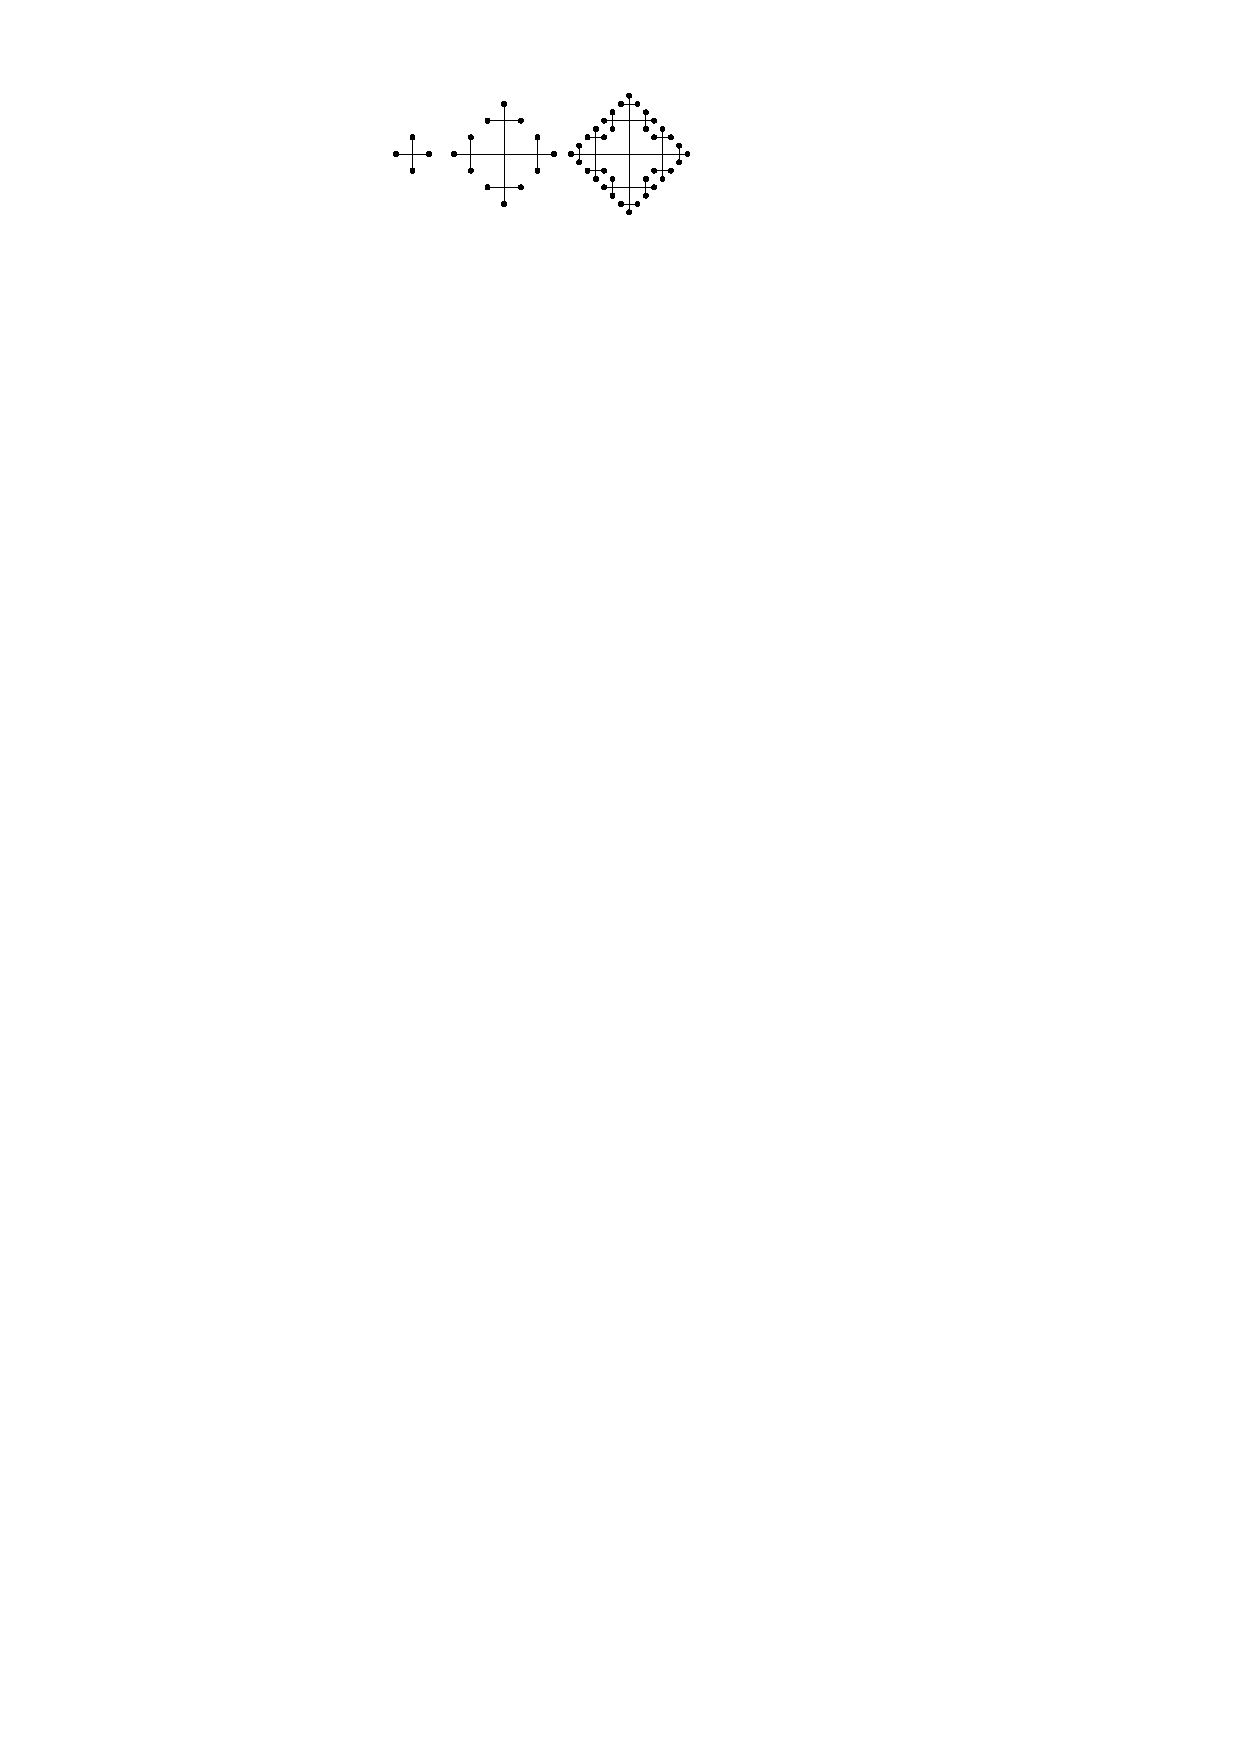
\includegraphics{free_group.pdf}}}$\lv{$a_n = 3 \cdot a_{n-1}$}%[scale=.8]
    \item $\vcenter{\hbox{
\includegraphics[height=1cm]{triangular_numbers.pdf}}}$\lv{$a_n = a_{n-1} + n$}
    \item $\vcenter{\hbox{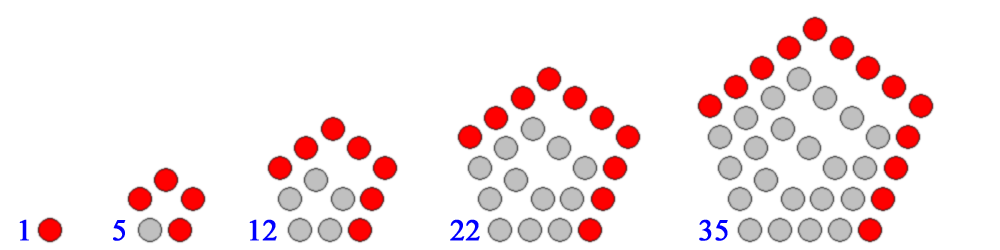
\includegraphics[height=2cm]{polygonal_number_5.png}}}$\lv{$a_n = a_{n-1} + 3n - 2$}
\end{enumerate*}
\end{flushleft}
\end{ulohav}


\interest
\begin{uloha}
Dokažte, že pro $n$-té Fibonacciho číslo $F_n$ (kde $F_1=F_2 = 1$) platí
\[ F_n = \frac{1}{\sqrt5}\left( \left( \frac{\sqrt5+1}{2} \right)^n - \left( \frac{1-\sqrt5}{2} \right)^n  \right). \]
\end{uloha}


\iinterest
\begin{uloha}
Kolik podmnožin množiny $\{1; 2; \dots; n\}$ má tu vlastnost, že neobsahuje dvě po sobě jdoucí čísla? Např. pro $n = 3$ jde o množiny $\{1\}$, $\{2\}$, $\{3\}$, $\{1; 3\}$ a prázdnou množinu (celkem pět podmnožin). Proč se tyto počty shodují s jinou známou posloupností?
\end{uloha}


\baselineskip=1.25\baselineskip
\setlist[enumerate]{label=\textbf{(\alph*)},itemjoin={\quad}}

\results
\parindent=0pt
\parskip=\smallskipamount
\rightskip=0pt plus1fil\relax
\def\printvysl#1#2{\textbf{#1.} #2\par}
\vysld
\endresults


\end{document}